\chapter{Correct-By-Construction System Dynamics}
\label{app:sd_simulation}

In this appendix we develop a correct-by-construction implementation of the SIR System Dynamics simulation. Note that the constant parameters \textit{populationSize, infectedCount, contactRate, infectivity, illnessDuration} are defined globally and omitted for clarity.

\section{Deriving the implementation}
Computing the dynamics of a SD model happens by taking the integrals as shown in Chapter \ref{sec:prop_sirspecs} and integrating over time. So conceptually we treat our SD model as a continuous function which is defined over time between 0 and infinity which outputs the values of each stock at each point in time. In the case of the SIR model we have 3 stocks: Susceptible, Infected and Recovered. Thus we start our implementation by defining the output of the SD function: for each time-step we have the values of the 3 stocks:

\begin{HaskellCode}
type SIRStep = (Time, Double, Double, Double)
\end{HaskellCode}

Next, we use a signal function to define the top-level function of the SIR SD simulation. It has no input, because an SD system is only defined by its own terms and parameters without external input and has as output the \textit{SIRStep}.

\begin{HaskellCode}
sir :: SF () SIRStep
\end{HaskellCode}

An SD model is fundamentally built on feedback: the values at time \textit{t} depend on the previous step. Thus, we introduce feedback in which we feed the last step into the next step. Yampa provides the \textit{loopPre :: c $\to$ SF (a, c) (b, c) $\to$ SF a b} function for that. It takes an initial value \textit{c} and a feedback signal function which receives the input \textit{a} and the previous (or initial) value of the feedback \textit{c} and has to return the output \textit{b} and the new feedback value \textit{c}. \textit{loopPre} then returns simply a signal function from \textit{a} to \textit{b} with the feedback happening transparent in the feedback signal function. The initial feedback value is the initial state of the SD model at $t = 0$. Further, we define the type of the feedback signal function.

\begin{HaskellCode}
sir = loopPre (0, initSus, initInf, initRec) sirFeedback
  where
    initSus = populationSize - infectedCount
    initInf = infectedCount
    initRec = 0
  
    sirFeedback :: SF ((), SIRStep) (SIRStep, SIRStep)
\end{HaskellCode}

The next step is to implement the feedback signal function. As input we get \textit{(a, c)} where \textit{a} is the empty tuple () because an SD simulation has no input, and \textit{c} is the fed back \textit{SIRStep} from the previous (initial) step. With this we have all relevant data so we can implement the feedback function. We first match on the tuple inputs and construct a signal function using \textit{proc}:

\begin{HaskellCode}
    sirFeedback = proc (_, (_, s, i, _)) -> do
\end{HaskellCode}

Now we define the flows which are \textit{infection rate} and \textit{recovery rate}. The formulas for both of them can be seen in the differential equations of Chapter \ref{sec:prop_sirspecs}. This directly translates into Haskell code:

\begin{HaskellCode}
infectionRate = (i * contactRate * s * infectivity) / populationSize
recoveryRate  = i / illnessDuration
\end{HaskellCode}

Next we need to compute the values of the three stocks, following the integral formulas of Chapter \ref{sec:prop_sirspecs}. For this we need the \textit{integral} function of Yampa which integrates over a numerical input using the rectangle rule. Adding initial values can be achieved with the \texttt{\string^<<} operator of arrowized programming. This directly translates into Haskell code:

\begin{HaskellCode}
s' <- (initSus+) ^<< integral -< (-infectionRate)
i' <- (initInf+) ^<< integral -< (infectionRate - recoveryRate)
r' <- (initRec+) ^<< integral -< recoveryRate
\end{HaskellCode}

We also need the current time of the simulation. For this we use Yampas \textit{time} function:

\begin{HaskellCode}
      t <- time -< ()
\end{HaskellCode}

Now we only need to return the output and the feedback value. Both types are the same thus we simply duplicate the tuple:

\begin{HaskellCode}
      returnA -< dupe (t, s', i', r')

    dupe :: a -> (a, a)
    dupe a = (a, a)
\end{HaskellCode}

We want to run the SD model for a given time with a given $\Delta t$ by running the \textit{sir} signal function. To \textit{purely} run a signal function Yampa provides the function \textit{embed :: SF a b $\rightarrow$ (a, [(DTime, Maybe a)]) $\rightarrow$ [b]} which allows to run an SF for a given number of steps where in each step one provides the $\Delta t$ and an input \textit{a}. The function then returns the output of the signal function for each step. Note that the input is optional, indicated by \textit{Maybe}. In the first step at $t = 0$, the initial \textit{a} is applied and whenever the input is \textit{Nothing} in subsequent steps, the last \textit{a} which was not \textit{Nothing} is re-used.

\begin{HaskellCode}
runSD :: Time -> DTime -> [SIRStep]
runSD t dt = embed sir ((), steps)
  where
    steps = replicate (floor (t / dt)) (dt, Nothing)
\end{HaskellCode}

\section{Results}
Although we have translated our model specifications directly into code we still need to validate the dynamics and test the system for its numerical behaviour under varying $\Delta t$. This is necessary because numerical integration, which happens in the \textit{integral} function, can be susceptible to instability and errors. Yampa implements the simple rectangle-rule of numerical integration which requires very small $\Delta t$ to keep the errors minimal and arrive at sufficiently good results. 

We have run the simulation with varying $\Delta t$ to show what difference varying $\Delta t$ can have on the simulation dynamics. We ran the simulations until $t = 100$ with a population Size $N$ = 1,000, contact rate $\beta = \frac{1}{5}$, infection probability $\gamma = 0.05$, illness duration $\delta = 15$ and initially 1 infected agent. For comparison we looked at the final values at $t = 100$ of the susceptible, infected and recovered stocks. Also, we compare the time and the value when the infected stock reaches its maximum. The values are reported in the Table \ref{tab:delta_influence}.

\begin{table}
  \centering
  \begin{tabular}{ c || c | c | c | c }
    $\Delta t$ & Susceptibles & Infected & Recovered & Max Infected \\ \hline \hline 
    1.0 & 17.52 & 26.87 & 955.61 & 419.07 @ t = 51 \\ \hline
    0.5 & 23.24 & 25.63 & 951.12 & 399.53 @ t = 47.5 \\ \hline
    0.1 & 27.56 & 24.27 & 948.17 & 384.71 @ t = 44.7 \\ \hline
    $1e-2$ & 28.52 & 24.11 & 947.36 & 381.48 @ t = 43.97 \\ \hline
    $1e-3$ & 28.62 & 24.08 & 947.30 & 381.16 @ t = 43.9  \\ \hline \hline
    AnyLogic & 28.625 & 24.081 & 947.294 & 381.132 @ t = 44
    
  \end{tabular}
  \caption{Results running the simulation with varying $\Delta t$ until $t = 100$ with a population Size $N$ = 1,000, contact rate $\beta = \frac{1}{5}$, infection probability $\gamma = 0.05$, illness duration $\delta = 15$ and initially 1 infected agent.}
  \label{tab:delta_influence}
\end{table}

As additional validation we added the results of a System Dynamics simulation in AnyLogic Personal Learning Edition 8.3.1, which is reported in the last row in the Table \ref{tab:delta_influence}. Also we provided a visualisation of the AnyLogics simulation dynamics in Figure \ref{fig:sir_sd_anylogic}. By comparing the results in Table \ref{tab:delta_influence} and the dynamics in Figure \ref{fig:sir_sd_anylogic} to \ref{fig:sir_sd_haskell_dynamics} we can conclude that we arrive at the same dynamics, validating the correctness of our simulation also against an existing, well-known and established System Dynamics software package.

\begin{figure}
\begin{center}
	\begin{tabular}{c}
		\begin{subfigure}[b]{1.0\textwidth}
			\centering
			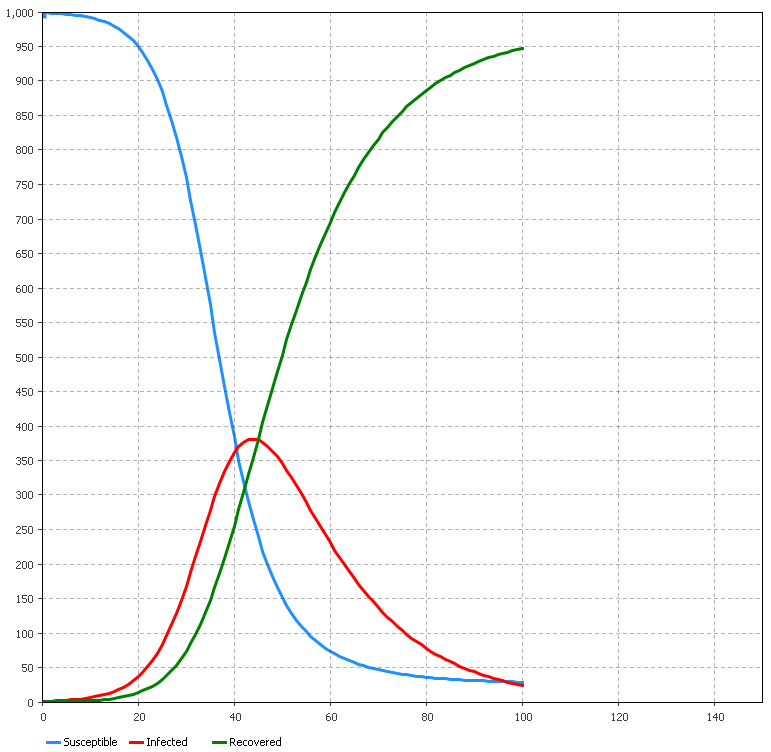
\includegraphics[width=.6\textwidth, angle=0]{./fig/appendix/sdsimulation/SIR_SD_1000agents_100t_ANYLOGIC.png}
			\caption{System Dynamics simulation of SIR compartment model in AnyLogic Personal Learning Edition 8.3.1. Population Size $N$ = 1,000, contact rate $\beta = \frac{1}{5}$, infection probability $\gamma = 0.05$, illness duration $\delta = 15$ with initially 1 infected agent. Simulation run until $t = 100$.}
	\label{fig:sir_sd_anylogic}
		\end{subfigure}
		
		\\
    	
		\begin{subfigure}[b]{1.0\textwidth}
			\centering
			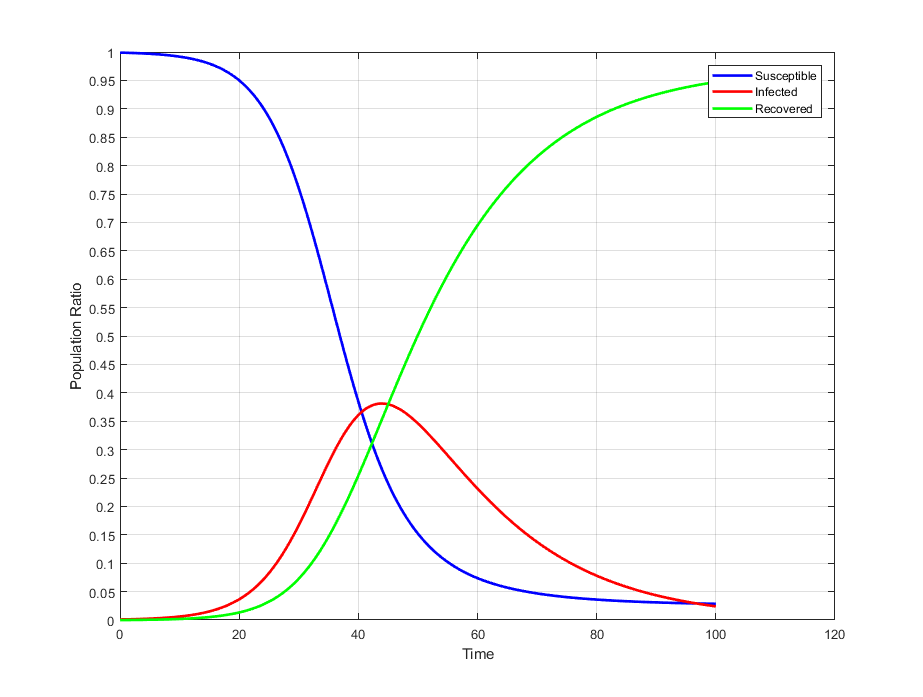
\includegraphics[width=.7\textwidth, angle=0]{./fig/appendix/sdsimulation/SIR_SD_1000agents_100t_0001dt.png}
			\caption{Dynamics of the SIR compartment model following this implementation. Population Size $N$ = 1,000, contact rate $\beta =  \frac{1}{5}$, infection probability $\gamma = 0.05$, illness duration $\delta = 15$ with initially 1 infected agent. Simulation run until $t = 150$. Plot generated from data by this Haskell implementation using Octave.}
			\label{fig:sir_sd_haskell_dynamics}
		\end{subfigure}
	\end{tabular}
	
	\caption{Visual comparison of the SIR SD dynamics generated by AnyLogic and our implementation in Haskell.} 
	\label{fig:sir_sd_haskell_vs_anylogic}
\end{center}
\end{figure}

\section{Discussion}
We claim that our implementation is correct-by-construction because the code \textit{is} the model specification - we have closed the gap between the specification and its implementation. Also we can guarantee that no non-deterministic influences can happen in this implementation due to the strong static type system of Haskell. This guarantees that repeated runs of the simulation will always result in the exact same dynamics given the same initial parameters, something of fundamental importance in System Dynamics.

%In this paper we have shown how to implement System Dynamics in a way that the resulting implementation is correct-by-construction, where the gap between the formal model specifications and the actual implementation in code is closed. We used the pure functional programming language Haskell for it and built on the Functional Reactive Programming concept to express our continuous-time simulation. The provided abstractions of Haskell and Functional Reactive Programming allowed to close the gap between the specification and implementation and further guarantee the absence of non-deterministic influences already at compile-time, making our correct-by-construction claims even stronger.

Further, we showed the influence of different $\Delta t$ and validated our implementation against the industry-strength System Dynamics simulation package AnyLogic Personal Learning Edition 8.3.1 where we could match our results with the one of AnyLogic, proving the correctness of our system also on the dynamics level.

Obviously the numerical well behaviour depends on the integral function which uses the rectangle rule. We showed that for the SIR model and small enough $\Delta t$, the rectangle rule works well enough. Still it might be of benefit if we provide more sophisticated numerical integration like Runge-Kutta methods. We leave this for further research.

The key strength of System Dynamic simulation packages is their visual representation which allows non-programmers to "draw" System Dynamics models and simulate them. We believe that one can auto-generate Haskell code using our approach to implement System Dynamics from such diagrams but leave this for further research.

Also we are very well aware that due to the vast amount of visual simulation packages available for System Dynamics, there is no big need for implementing such simulations directly in code. Still we hope that our pure functional approach with Functional Reactive Programming might spark an interest in approaching the implementation of System Dynamics from a new perspective, which might lead to pure functional back-ends of visual simulation packages, giving them more confidence in their correctness.

\newpage

\section{Full Implementation}

\begin{HaskellCode}
populationSize :: Double
populationSize = 1000

infectedCount :: Double
infectedCount = 1

contactRate :: Double
contactRate = 5

infectivity :: Double
infectivity = 0.05

illnessDuration :: Double
illnessDuration = 15

type SIRStep = (Time, Double, Double, Double)

sir :: SF () SIRStep
sir = loopPre (0, initSus, initInf, initRec) sirFeedback
  where
    initSus = populationSize - infectedCount
    initInf = infectedCount
    initRec = 0

    sirFeedback :: SF ((), SIRStep) (SIRStep, SIRStep)
    sirFeedback = proc (_, (_, s, i, _)) -> do
      let infectionRate = (i * contactRate * s * infectivity) / populationSize
          recoveryRate  = i / illnessDuration

      t <- time -< ()

      s' <- (initSus+) ^<< integral -< (-infectionRate)
      i' <- (initInf+) ^<< integral -< (infectionRate - recoveryRate)
      r' <- (initRec+) ^<< integral -< recoveryRate

      returnA -< dupe (t, s', i', r')

    dupe :: a -> (a, a)
    dupe a = (a, a)

runSD :: Time -> DTime -> [SIRStep]
runSD t dt = embed sir ((), steps)
  where
    steps = replicate (floor (t / dt)) (dt, Nothing)
\end{HaskellCode}